% Copyright 2004 by Till Tantau <tantau@users.sourceforge.net>.
%
% In principle, this file can be redistributed and/or modified under
% the terms of the GNU Public License, version 2.
%
% However, this file is supposed to be a template to be modified
% for your own needs. For this reason, if you use this file as a
% template and not specifically distribute it as part of a another
% package/program, I grant the extra permission to freely copy and
% modify this file as you see fit and even to delete this copyright
% notice. 

%\documentclass[11pt,aspectratio=169]{beamer}
\documentclass[11pt,aspectratio=43]{beamer}
\setbeamercovered{transparent}
\usepackage{epsfig, subfigure, amssymb, multirow, algorithmic, amsmath}
\usepackage[default]{lato}
\usepackage[T1]{fontenc}
\usepackage{caption}
\usepackage[ruled, linesnumbered, vlined]{algorithm2e}

\captionsetup{font=scriptsize,labelfont=scriptsize}

% There are many different themes available for Beamer. A comprehensive
% list with examples is given here:
% http://deic.uab.es/~iblanes/beamer_gallery/index_by_theme.html
% You can uncomment the themes below if you would like to use a different
% one:
%\usetheme{AnnArbor}
%\usetheme{Antibes}
%\usetheme{Bergen}
%\usetheme{Berkeley}
%\usetheme{Berlin}
%\usetheme{Boadilla}
%\usetheme{boxes}
%\usetheme{CambridgeUS}
%\usetheme{Copenhagen}
%\usetheme{Darmstadt}
%\usetheme{default}
%\usetheme{Frankfurt}
%\usetheme{Goettingen}
%\usetheme{Hannover}
%\usetheme{Ilmenau}
%\usetheme{JuanLesPins}
%\usetheme{Luebeck}
\usetheme{Madrid}
%\usetheme{Malmoe}
%\usetheme{Marburg}
%\usetheme{Montpellier}
%\usetheme{PaloAlto}
%\usetheme{Pittsburgh}
%\usetheme{Rochester}
%\usetheme{Singapore}
%\usetheme{Szeged}
%\usetheme{Warsaw}

\usepackage{lmodern}
\definecolor{colorA}{RGB}{1, 66, 96}
\definecolor{colorB}{RGB}{26, 26, 26}
% Change base colour beamer@blendedblue (originally RGB: 0.2,0.2,0.7)
\colorlet{beamer@blendedblue}{colorA!40!colorB}

\title[{PET/CT Denoising and Segmentation }]{\textbf{PET/CT Image Denoising and Segmentation based on a Multi Observation and Multi Scale Markov Tree Model}}

% A subtitle is optional and this may be deleted
\subtitle{\textit{[Medical Sensors Defense]}}

\author{Yeman Hagos \and Vu Hoang Minh}
% - Give the names in the same order as the appear in the paper.
% - Use the \inst{?} command only if the authors have different
%   affiliation.

\institute[] % (optional, but mostly needed)
{
  University of Bourgogne
  }
% - Use the \inst command only if there are several affiliations.
% - Keep it simple, no one is interested in your street address.

\date{November 25, 2016}
% - Either use conference name or its abbreviation.
% - Not really informative to the audience, more for people (including
%   yourself) who are reading the slides online

\subject{Theoretical Computer Science}
% This is only inserted into the PDF information catalog. Can be left
% out. 

% If you have a file called "university-logo-filename.xxx", where xxx
% is a graphic format that can be processed by latex or pdflatex,
% resp., then you can add a logo as follows:

% \pgfdeclareimage[height=0.5cm]{university-logo}{university-logo-filename}
% \logo{\pgfuseimage{university-logo}}

% Delete this, if you do not want the table of contents to pop up at
% the beginning of each subsection:
\AtBeginSection[]
{
  \begin{frame}<beamer>{Outline}
    \tableofcontents[currentsection]
  \end{frame}
}



\begin{document}

%========================
% title and outline
%========================
\begin{frame}
  \titlepage
\end{frame}

\begin{frame}{Outline}
  \tableofcontents
  % You might wish to add the option [pausesections]
\end{frame}

%========================
% main content
%========================
\section{Introduction}



\section{Literature Review}
\subsection{Hidden Markov Tree}
\begin{frame}
	\frametitle{Hidden Markov Tree}		
\end{frame}
\subsection{Wavelet Transform}
\subsection{Contourlet Transform}
\subsection{PET Denoising}
\subsection{PET/CT Segmentation}
\section{Result}
\section{Conclusion}




%\section{Lists}
% --------------------------------------------------- Slide --
%\subsection{Itemize}
\label{itemize}
\begin{frame}\frametitle{Lists - Itemize}
  \begin{itemize}
    \item Point A
    \item Point B
    \begin{itemize}
      \item part 1
      \item part 2
    \end{itemize}
    \item Point C
    \item Point D
  \end{itemize}
\end{frame}

% --------------------------------------------------- Slide --
%\subsection{Pause}
\label{pause}
\begin{frame}\frametitle{Lists - Itemize with Pause}
  \begin{itemize}
    \pause \item Point A
    \pause \item Point B
    \begin{itemize}
      \pause \item part 1
      \pause \item part 2
    \end{itemize}
    \pause \item Point C
    \pause \item Point D
  \end{itemize}
\end{frame}

% --------------------------------------------------- Slide --
%\subsection{Enumerate}
\label{enumerate}
\begin{frame}\frametitle{Lists - Enumerate}
  \begin{enumerate}
    \item Point A
    \item Point B
    \begin{enumerate}
      \item part 1
      \item part 2
    \end{enumerate}
    \item Point C
    \item Point D
  \end{enumerate}
\end{frame}

% --------------------------------------------------- Slide --
%\subsection{Enumerate (Roman Numerals)}
\label{enumerateRomanNumerals}
\begin{frame}\frametitle{Lists - Enumerate (Roman Numerals)}
  \begin{enumerate} [(I)]
	\item Point A
	\item Point B
	\begin{enumerate} [(i)]
	  \item part 1
      \item part 2
	\end{enumerate}
	\item Point C
	\item Point D
  \end{enumerate}
\end{frame}
%\section{Columns}
% --------------------------------------------------- Slide --
%\subsection{Columns}
\label{columns}
\begin{frame}\frametitle{Columns}
  \begin{columns}
    \column{0.5\textwidth}
      Lorem ipsum dolor sit amet, consectetur adipisicing elit, sed do eiusmod tempor incididunt ut labore et dolore magna aliqua.
    \column{0.5\textwidth}
      Lorem ipsum dolor sit amet, consectetur adipisicing elit, sed do eiusmod tempor incididunt ut labore et dolore magna aliqua.
  \end{columns}
\end{frame}
%%\section{Figures}
% --------------------------------------------------- Slide --
%\subsection{Figures}
\label{figures}
\begin{frame}\frametitle{Domination on a Chessboard}
  \begin{figure}[htb]
    \centering
    \begin{tabular}{cc}\pause{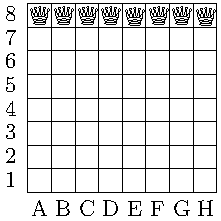
\includegraphics[scale=1]{examples/DomChess8.pdf}}&
      \pause{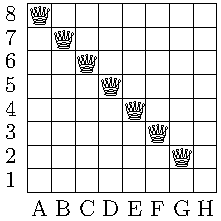
\includegraphics[scale=1]{examples/DomChess7.pdf}}\\
      \pause{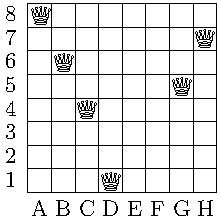
\includegraphics[scale=1]{examples/DomChess6.pdf}}&
      \pause{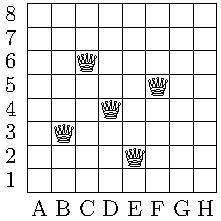
\includegraphics[scale=1]{examples/Chess1.pdf}}
    \end{tabular}
  \end{figure}
\end{frame}

% --------------------------------------------------- Slide --
%\subsection{Figures}
\label{figures2}
\begin{frame}\frametitle{Single figure with caption}
  \begin{figure}[htb]
    \centering
    
\includegraphics[scale=0.25]{examples/figures/400x400.png}
    \caption{This is an caption!}
  \end{figure}
\end{frame}
%\section{Description}
% --------------------------------------------------- Slide --
%\subsection{Description}
\label{description}
\begin{frame}\frametitle{Description Environment}
  \begin{description}
    \item[API] Application Programming Interface
    \item[LAN] Local Area Network
    \item[ASCII] American Standard Code for Information Interchange
  \end{description}
\end{frame}
%\section{Tables}
% --------------------------------------------------- Slide --
%\subsection{Tables}
\label{tables}
\begin{frame}\frametitle{Tables}
  \begin{table}
    \begin{tabular}{l | c | c | c | c }
      Competitor Name & Swim & Cycle & Run & Total \\
      \hline \hline
      John T & 13:04 & 24:15 & 18:34 & 55:53 \\ 
      Norman P & 8:00 & 22:45 & 23:02 & 53:47\\
      Alex K & 14:00 & 28:00 & n/a & n/a\\
      Sarah H & 9:22 & 21:10 & 24:03 & 54:35 
    \end{tabular}
    \caption{Triathlon results}
  \end{table}
\end{frame}
%\section{Blocks}
% --------------------------------------------------- Slide --
%\subsection{Blocks}
\label{blocks}
\begin{frame}\frametitle{Blocks}
  \begin{block}{Block Title}
    Lorem ipsum dolor sit amet, consectetur adipisicing elit, sed do eiusmod tempor incididunt ut labore et dolore magna aliqua.
  \end{block}
  \begin{alertblock}{Alert Block Title}
    Lorem ipsum dolor sit amet, consectetur adipisicing elit, sed do eiusmod tempor incididunt ut labore et dolore magna aliqua.
  \end{alertblock}
\end{frame}
%\section{Definition}
% --------------------------------------------------- Slide --
%\subsection{Definition}
\label{definition}
\begin{frame}\frametitle{Definition}
  Then there’s the definition environment which produces a standard ColorA color block but with the title already specified as ‘definition’.
  \begin{semiverbatim}
    \\begin\{definition\}\newline
    A prime number is a number that...\newline
    \\end\{definition\}
  \end{semiverbatim}
  \begin{definition}
    A prime number is a number that...
  \end{definition}
\end{frame}
%\section{Example}
% --------------------------------------------------- Slide --
%\subsection{Example}
\label{example}
\begin{frame}\frametitle{Example}
  Next there’s the example environment which produces a green block with the title ‘Example’.
  \begin{semiverbatim}
    \\begin\{example\}\newline
    Lorem ipsum dolor sit amet...\newline
    \\end\{example\}
  \end{semiverbatim}
  \begin{example}
    Lorem ipsum dolor sit amet, consectetur adipisicing elit, sed do eiusmod tempor incididunt ut labore et dolore magna aliqua.
  \end{example} 
\end{frame}
%\section{Theorem}
% --------------------------------------------------- Slide --
%\subsection{Theorem Code}
\label{theoremCode}
\begin{frame}\frametitle{Theorem}
  There is also a group of blocks that are especially useful for presenting mathematics. For example the ‘theorem’ environment, the ‘corollary’ environment and the ‘proof’ environment.
  \begin{semiverbatim}
    \\begin\{theorem\}[Pythagoras] \newline
      $ a^2 + b^2 = c^2$ \newline
    \\end\{theorem\} \newline
    \\begin\{corollary\} \newline
      $ x + y = y + x  $ \newline
    \\end\{corollary\} \newline
    \\begin\{proof\} \newline
      $\omega +\phi = \epsilon $ \newline
    \\end\{proof\}
  \end{semiverbatim}
\end{frame}

% --------------------------------------------------- Slide --
%\subsection{Theorem Blocks}
\label{theoremBlocks}
\begin{frame}\frametitle{Theorem Blocks}
  \begin{theorem}[Pythagoras] 
    $ a^2 + b^2 = c^2$
  \end{theorem}
  \begin{corollary}
    $ x + y = y + x  $
  \end{corollary}
  \begin{proof}
    $\omega +\phi = \epsilon $
  \end{proof}
\end{frame}
%\section{Hyperlinks}
% --------------------------------------------------- Slide --
%\subsection{Hyperlinks Code}
\label{hyperlinks}
\begin{frame}\frametitle{Hyperlink}
Before we can create any hyperlinks we need to tag the frames we want to link to using the \label command.
 
\hyperlink{contents}{click here}
\hyperlink{section1}{\beamerbutton{section 1 page}}
\hyperlink{columns}{\beamergotobutton{columns page}}
\hyperlink{pictures}{\beamerskipbutton{pictures page}}
\hyperlink{pictures}{\beamerreturnbutton{pictures page}}

\end{frame}
\SetKwInOut{Input}{Input}\SetKwInOut{Output}{Output}
\begin{frame}\frametitle{A trivial Set Cover algorithm}
\begin{algorithm}[H]\footnotesize
        \Input{A set cover instance $({\cal S,U})$ and a variable ${\cal S}_{\rm dom}$.}
        \Output{A minimum set cover of $({\cal S,U})$.}
\If{${\cal S}=\emptyset$}{
\Return $\emptyset$\;
}
Let $S \in {\cal{S}}$ be a set of maximum cardinality\;
${\cal{C}}_1 = \{S\}\cup {\tt MSC}(\{S'\backslash S \mid S' \in{\cal S}\backslash \{S\}\}, {\cal U}\backslash S )$\;
${\cal{C}}_2 = {\tt MSC}({\cal S}\backslash \{S\},{\cal U})$\;
${\cal S}_{\rm dom} \leftarrow \emptyset$\;
\If{${\cal U} \subseteq {\cal C}_1$}{
${\cal S}_{\rm dom} \leftarrow {\cal C}_1$\;
\If{${\cal U} \subseteq {\cal C}_2$}{
\If{$|{\cal C}_2| < |{\cal C}_1|$}{
${\cal S}_{\rm dom} \leftarrow {\cal C}_2$\;
}
}
}
\Return ${\cal S}_{\rm dom}$\;
\caption{{\tt MSC}$({\cal S,U})$}
\end{algorithm}
\end{frame}


%========================
% qa and thank you
%========================
\begin{frame}
	\centering
	\huge{Q \& A}	
\end{frame}

\begin{frame}
	\centering
	\huge{Thank you for listening}	
\end{frame}

\end{document}


